\documentclass[journal]{IEEEtran}
\usepackage{graphicx}
\usepackage{amsmath,amsthm,amssymb} 
\usepackage{subcaption}
\usepackage{tikz}

\newcommand{\norm}[1]{\left\lVert#1\right\rVert}

\begin{document}
\title{Street View House Numbers Recognition}
\maketitle

\begin{abstract}
We used three different machine learning algorithms, including Logistic Regression, Neural Network and Convolutional Neural Network to recognize digits from Street View House Numbers data set\footnote{http://ufldl.stanford.edu/housenumbers/}.
We implemented the algorithms with Tensorflow\footnote{https://www.tensorflow.org/}, and compared their performance, as well as pros and cons. Wel also implemented SimpleNet\cite{simplenet} for comparison with our models.
\end{abstract}

\section{Introduction}

Character recognition can be considered as a solved task, especially after the concept of CNN is formalized by LeCun et.al.\cite{lecun1998}. Character recognition in the natural scene is a much harder problem due to the high flexibility 
of input. A typical example is the SVHN (Street View House Numbers) data set. This data set consists of 73257 training images and 26032 test images obtained
from Google Street View images(Figure \ref{fig:svhn_sample}), each of which is $32 \times 32$ with RGB channels. Based on benchmark.ai\footnote{https://benchmarks.ai/svhn}, the state-of-the-art solution from Cubuk et.al.\cite{cubuk2018} achieved 1.02\% error rate.

In this project we studied the performance of three different algorithms on SVHN dataset, namely, Logistic Regression, Feedforward Neural Network, and Convolutional Neural Network, compared their performance, and discussed their pros and cons. For comparison purpose we also implemented SimpleNet \cite{simplenet}.

We conclude that SVHN dataset is not linearly separable, thus linear model such as Logistic Regression will not generate an acceptable performance. Non-linear models such as Feedforward Neural Network is able to achieve a decent result, while a deep Convolutional Neural Network can extract image features more efficiently and generate much better performance.

\begin{figure}[!t]
    \centering
    \includegraphics[width=.45\textwidth]{images/32x32eg.png}
    \caption{32$\times$32 cropped samples from SVHN data set.}
    \label{fig:svhn_sample}
\end{figure}


\section{Algorithms}

To simplify coding, we implemented an interface inspired by Keras. With this interface, a neural network can be created by simply stacking the layers, without considering the tensor connections between layers.

\subsection{Logistic Regression}

Logistic Regression is one of the traditional machine learning algorithms and is the most commonly implemented by machine learning and statistical software packages. 

The preprocessed input images are $32 \times 32$ with 1 channel, thus the data shape is $32 \times 32 \times 1$. In order to use in logistic regression, an input image is flattened into one single vector with $D = 1024$ dimensions. The output consists of $K = 10$ classes. We apply logistic regression to the input to compute the loss:
$$\mathcal{L}(\mathbf{w}, b) = \theta(\mathbf{w}^\intercal \mathbf{x} + b)$$,
where $\mathbf{w} \in \mathbb{R}^{D \times K}, b \in \mathbb{R}^{K}$, and $\sigma(z)_i = e^{\sigma_i} / \sum_{k=1}^K e^{\theta_k}$ is the softmax function.

L2 regularization is used to avoid overfitting. Thus the loss function can be written as:
$$\mathcal{L}(\mathbf{w}, b) = \theta(\mathbf{w}^\intercal \mathbf{x} + b) + \lambda \norm{\textbf{w}}$$

In this project we choose to implement Logistic Regression with Tensorflow. since logistic regression is equivalent to the \texttt{Dense} layer in neural network, we can reuse the neural network code. A \texttt{Flatten} layer reshapes the input images to vector then a \texttt{Dense} layer will apply the Logistic Regression.

\subsection{Neural Network}

Neural network is usually referred as ``multiple layer perceptron'' (or MLP) as it uses one or more ``hidden layers''. Neural network can simulate non-linear models of any complexity.

For this project, we used a simple network with only one hidden layer with 1024 hidden units.
Similar to Logistic Regression, the input images are reshaped to vectors with $D=1024$. 
Figure \ref{fig:nn_arch} shows the architecture of the neural network we used.

\begin{figure}[tb]
    \centering
    

\tikzset{every picture/.style={line width=0.75pt}} %set default line width to 0.75pt        

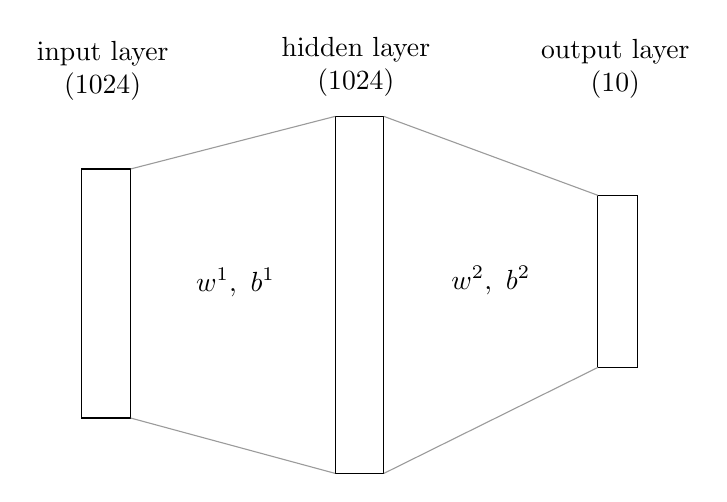
\begin{tikzpicture}[x=0.75pt,y=0.75pt,yscale=-1,xscale=1]
%uncomment if require: \path (0,300); %set diagram left start at 0, and has height of 300

%Shape: Rectangle [id:dp6149643085998178] 
\draw   (54,93.33) -- (77.5,93.33) -- (77.5,213.33) -- (54,213.33) -- cycle ;
%Shape: Rectangle [id:dp5092925997669449] 
\draw   (176,68) -- (199.5,68) -- (199.5,240) -- (176,240) -- cycle ;
%Straight Lines [id:da7027489864850467] 
\draw [color={rgb, 255:red, 155; green, 155; blue, 155 }  ,draw opacity=1 ]   (77.5,93.33) -- (176,68) ;


%Straight Lines [id:da30180540366043385] 
\draw [color={rgb, 255:red, 155; green, 155; blue, 155 }  ,draw opacity=1 ]   (77.5,213.33) -- (176,240) ;


%Shape: Rectangle [id:dp4986098264860639] 
\draw   (302.5,106) -- (321.5,106) -- (321.5,189) -- (302.5,189) -- cycle ;
%Straight Lines [id:da45051042505798455] 
\draw [color={rgb, 255:red, 155; green, 155; blue, 155 }  ,draw opacity=1 ]   (199.5,68) -- (302.5,106) ;


%Straight Lines [id:da9299225224259415] 
\draw [color={rgb, 255:red, 155; green, 155; blue, 155 }  ,draw opacity=1 ]   (199.5,240) -- (302.5,189) ;



% Text Node
\draw (128,148) node  [align=left] {$\displaystyle w^{1} ,\ b^{1}$};
% Text Node
\draw (251,147) node  [align=left] {$\displaystyle w^{2} ,\ b^{2}$};
% Text Node
\draw (186,44) node  [align=center] {hidden layer\\(1024)};
% Text Node
\draw (64,46) node  [align=center] {input layer\\(1024)};
% Text Node
\draw (311,45) node  [align=center] {output layer\\(10)};


\end{tikzpicture}

    \caption{Neural Network Architecture.}
    \label{fig:nn_arch}
\end{figure}

\subsection{Convolutional Neural Network}

Convolutional Neural Network (or CNN) is a class of deep neural networks most applied to image recognition tasks. A typical CNN includes the following types of layers:

\begin{itemize}
    \item Convolutiona layer: This type of layers apply convolution operation to the input. Convolution operation produces less parameters than simple fully connected layer.
    \item Pooling layer: Pooling layers reduce the dimension of the input by combining adjacent outputs. The most common pooling layer is max pooling.
    \item Fully Connected layer: A fully connected layer is the same layer as in multiple layer perceptron network. This type of layers are usually used after the input data is flattened to produce output for prediction.
\end{itemize}

For CNN we used an architecture consists of one convolutional layer and one subsampling layer.
For comparison, we also implemented Simplet\cite{simplenet} in Tensorflow.
Table \ref{table:cnn_arch} shows the architecture of the CNN and SimpleNet.

\begin{table}[htb]
\centering
\begin{tabular}{l|l}
\hline
CNN & SimpleNet \\
\hline
conv2d(32/3x3), relu, bn & conv2d(64/3x3), bn, relu \\
 & [conv2d(32/3x3, bn, relu] x 3  \\
max\_pooling(2x2) & max\_pooling(2x2) \\
& [conv2d(32/3x3), bn, relu] x 2 \\
& conv2d(64/3x3), bn, relu \\
& max\_pooling(2x2) \\
& [conv2d(64/3x3), bn, relu] x 2 \\
& max\_pooling(2x2) \\
& conv2d(128/3x3), bn, relu \\
& conv2d(256/1x1), bn, relu \\
& conv2d(64/1x1), bn, relu \\
& max\_pooling(2x2) \\
& conv2d(64/3x3), bn, relu \\
& max\_pooling(2x2) \\
flatten & flatten  \\
dense(1024) &  \\
dropout(0.5) &  \\
dense(10) & dense(10) \\
\hline
\end{tabular}
\caption{Convolutional Neural Network Architecture. ``bn`` is batch normalization layer. CNN uses input moment as batch normalization parameter, and SimpleNet uses batch normalization with decay=0.95. The number in ``[layers] x 3'' denotes repetition of the layers.}
\label{table:cnn_arch}
\end{table}

\section{Experiments and Analysis}

\textbf{Data Preprocessing.} Before applying algorithms, we preprocessed the data set by first converting images from RGB to grayscale, then executing an auto contrast, in order to keep the contrast of images at the same level. The preprocessed images are shown in Figure \ref{fig:preprocessed_images}.

\begin{figure}[t]
    \centering
    \includegraphics[width=.5\textwidth]{images/preprocessed_svhn.png}
    \caption{Preprocessed images of digits 0 - 9.}
    \label{fig:preprocessed_images}
\end{figure}

\textbf{Dynamic Learning Rate.} During the experiment, we realized that choosing an appropriate learning rate is critical for the performance of neural network. However a very small learning rate will increase the training time significantly. Thus we decide to use dynamic learning rate which decreases  exponentially. Concretely, the learning rate starts with $0.001$, and decreases to $1/10$ every 100 epochs. This dynamic learning rate played an important role in the training, as illustrated later in Figure \ref{fig:cnn_loss} and \ref{fig:simplenet_loss}.

We trained each model with the train data for 400 epochs, and plotted the training/test error every 10 epochs. Figure \ref{fig:lr_loss}, \ref{fig:nn_loss}, and \ref{fig:cnn_loss} show the loss and error for each model respectively. Table \ref{table:loss_error} shows the loss and error rate at epoch 400.

Note that for SimpleNet we trained two versions, without dropout and with dropout respectively. This will be disscussed in detail in Section \ref{section:simplenet}.

\begin{table}[htb]
\centering
\begin{tabular}{c|r|r|r|r}
\hline
model & train loss & test loss & train err & test err \\ \hline
Logistic & 2.1448 & 2.2447 & 71.06\% & 74.18\% \\
NN & 0.5280 & 0.6798 & 7.86\% & 13.51\% \\
CNN & 0.2314 & 0.5987 & 3.02\% & 13.78\% \\
SimpeNet(w/o dropout) & 0.0055 & 0.2982 & 0.00\% & 5.50\% \\
SimpeNet(w/ dropout) & 0.0546 & 0.1982 & 0.13\% & 3.38\% \\
\hline
\end{tabular}
\caption{Loss and error rate at epoch 400.}
\label{table:loss_error}
\end{table}

\subsection{Logistic Regression}

Figure \ref{fig:lr_loss} shows the loss and error rate of Logistic Regression. At epoch 400 the test error rate is 74.18\%. The optimization converges after 200 epoch, and from the error plot we can see that there is no significant raise in test error, indicating that overfitting is not happening.

Figure \ref{fig:lr_cm} shows the confusion matrix of Logistic Regression.
Most digits are predicted as ``1'', ``2'', and ``5'', while complicated digits such as
``3'', ``4'', ``7'', and ``9'' have almost no prediction.

Therefore, we conclude that the linear model is overly simple that underfit this dataset.

\begin{figure}[htb]
\minipage{0.24\textwidth}
  \includegraphics[width=\linewidth]{images/lr-loss.png}
\endminipage\hfill
\minipage{0.24\textwidth}
  \includegraphics[width=\linewidth]{images/lr-error.png}
\endminipage
\caption{Loss(left) and error rate(right) in training and test phase, for Logistic Regression model.}\label{fig:lr_loss}
\end{figure}

\begin{figure}[htb]
\includegraphics[width=\linewidth]{images/lr-cm.png}
\caption{Confusion matrix for Logistic Regression.}\label{fig:lr_cm}
\end{figure}

\subsection{Feedforward Neural Network}

Figure \ref{fig:nn_loss} shows the loss and error rate of Feedforward Neural Network. This model is able to fit the non-linear nature of the data set and produced a decent performance with 13.51\% error rate.

However, neural network need much more free parameters.
In our model, the hidden layer has 1024 hidden units which requires $1024 \times 1024$ free parameters, and output layer requires $1024 \times 10$ parameters, in total approximately 1M parameters are required.

\begin{figure}[htb]
\minipage{0.24\textwidth}
  \includegraphics[width=\linewidth]{images/nn-loss.png}
\endminipage\hfill
\minipage{0.24\textwidth}
  \includegraphics[width=\linewidth]{images/nn-error.png}
\endminipage
\caption{Loss(left) and error rate(right) in training and test phase, for Feedforward Neural Network model.}\label{fig:nn_loss}
\end{figure}

\begin{figure}[htb]
\includegraphics[width=\linewidth]{images/nn-cm.png}
\caption{Confusion matrix for Feedforward Neural Network.}\label{fig:nn_cm}
\end{figure}


\subsection{Convolutional Neural Network}

Figure \ref{fig:cnn_loss} shows the loss and error rate of Convolutional Neural Network. The performance (error rate ??) is similar to Feedforward Neural Network, however it requires much less free parameters. In our CNN model, convolution layer has $3 \times 3 \times 32 = 288$ parameters, the first dense layer has $16 \times 16 \times 128 = 32768$ parameters, and the output layer has $128 * 10 = 1280$ parameters, in total approximately 33k parameters are required. Compared to the 1M parameters in feedforward neural network, this is a great improvement and can reduce the model complexity significantly.

During the training process we can also see that dynamic learning rate is important. The first converge occurred around 50 epochs, from where the loss became unstable, 
which indicates our initial learning rate 0.001 became too large.
At epoch 100, the learning rate decreased to 0.0001,
and the optimization continued. This shows that our dynamic learning rate approach worked well in this training, enabled our CNN model to achieve a better performance.


\begin{figure}[htb]
\minipage{0.24\textwidth}
  \includegraphics[width=\linewidth]{images/cnn-loss.png}
\endminipage\hfill
\minipage{0.24\textwidth}
  \includegraphics[width=\linewidth]{images/cnn-error.png}
\endminipage
\caption{Loss(left) and error rate(right) in training and test phase, for Convolutional Neural Network model.}\label{fig:cnn_loss}
\end{figure}

\begin{figure}[htb]
\includegraphics[width=\linewidth]{images/cnn-cm.png}
\caption{Confusion matrix for Convolutional Neural Network.}\label{fig:cnn_cm}
\end{figure}

\subsection{SimpleNet}\label{section:simplenet}

Among the four models in this project, SimpleNet(Figure \ref{fig:simplenet_loss}) achieved the best performance, with test error rate 5.50\% at epoch 400. This can be considered that it is a deep convolutional neural network that consists of enough free parameters to ``remember'' more patterns in the input images.

Our dynamic learning rate strategy also has a significantly positive effect that it enabled further optimization at epoch 100 and 200.

We also observed that while training error stays stable after 200 epoch, test error starts to rise. This indicates that overfitting happened after epoch 200. To reduce overfitting, we then added a dropout layer with keep probability 0.8 after the ReLU function of each convolution layer. Figure \ref{fig:simplenet-dropout_loss} shows that after applying dropout, the train error (0.13\%) is higher than the model without dropout (approximately 0.00\%), however it generalizes better, with test error (3.38\%) lower than the model without dropout (5.50\%). This shows that dropout can successfully prevent overfitting and eventually increase the prediction accuracy.

The confusion matrix for SimpleNet in Figure \ref{fig:simplenet-dropout_cm} shows the SimpleNet can classify the data set correctly.

\begin{figure}[htb]
\minipage{0.24\textwidth}
  \includegraphics[width=\linewidth]{images/simplenet-loss.png}
\endminipage\hfill
\minipage{0.24\textwidth}
  \includegraphics[width=\linewidth]{images/simplenet-error.png}
\endminipage
\caption{Loss(left) and error rate(right) in training and test phase, for SimpleNet(without dropout).}\label{fig:simplenet_loss}
\end{figure}

\begin{figure}[htb]
\minipage{0.24\textwidth}
  \includegraphics[width=\linewidth]{images/simplenet-dropout-loss.png}
\endminipage\hfill
\minipage{0.24\textwidth}
  \includegraphics[width=\linewidth]{images/simplenet-dropout-error.png}
\endminipage
\caption{Loss(left) and error rate(right) in training and test phase, for SimpleNet(with dropout).}\label{fig:simplenet-dropout_loss}
\end{figure}


\begin{figure}[htb]
\includegraphics[width=\linewidth]{images/simplenet-cm.png}
\caption{Confusion matrix for SimpleNet(with dropout).}\label{fig:simplenet-dropout_cm}
\end{figure}


\section{Conclusion}

In this project we implemented three models: Logistic Regression, Feedforward Neural Network, and Convolutional Neural Network, and tested their performance on SVHN dataset.
As a comparison, we also implemented SimpleNet, without dropout and with dropout.

What we have learned from this project:
\begin{itemize}
\item Logistic Regression does not perform well on complex data set due to its simplicity;
\item Feedforward Neural Network can simulate any non-linear model thus is able to classify non-linear dataset; However the fully connected hidden layers require too many free parameters which causes slow training and huge storage requirement;
\item Convolutional Neural Network uses convolution operation to extract features automatically from the input images, thus is able to achieve same or better performance than Feedforward Neural Network with less computational power.
It also requires less parameters.
\item Deep Convolutional Neural Network can achieve astonishing good performance, since it has more layers and parameters to learn more features from input images. However it is prone to overfitting, thus techniques to prevent overfitting such as batch normalization and dropout are usually necessary.
\end{itemize}

\begin{thebibliography}{9}
    \raggedright
    \bibitem{lecun1998}
    Y. LeCun, L. Bottou, Y. Bengio, and P. Haffner. \emph{Gradient-based learning applied to document recognition.} Proceedings of the IEEE, november 1998.

    \bibitem{cubuk2018}
    Ekin D. Cubuk et.al. \emph{AutoAugment: Learning Augmentation Policies from Data}, arXiv:1805.09501
    
    \bibitem{simplenet}
    Seyyed H. Hasanpour et.al. \emph{Lets keep it simple, Using simple architectures to outperform deeper and more complex architectures}, arXiv:1608.06037
\end{thebibliography}


\end{document}
